\subsection{检测效果分析}
\label{subsec:featurespy-evaluation-detection}



\paragraph*{Exp\#1(明文块的相似性检测)。}
我们首先证明我们可以通过比较内容特征来有效地找到相似的明文块。 我们考虑多个 SYNChunk$(x, y)$,每个 SYNChunk$(x, y)$ 包括 10\,K 个从基本块修改的相似块(即 ground truth)(回想一下,$x$ 定义了修改位置的数量,$y$ 定义每个位置的修改字节数,参见\S\ref{subsec:featurespy-datasets})。 我们为 SYNChunk$(x, y)$ 中的每个明文块提取四个内容特征,如果它们分别共享一到四个相同的特征,则识别相似的块。 我们评估在基本事实中的所有(相似)块中成功识别的相似块的比例。


\begin{figure}[t]
    \centering
    
\includegraphics[width=0.4\textwidth]{pic/featurespy/plot/detection/syn/fixed_pq_legend.pdf}
    \vspace{5pt}\\
    \begin{tabular}{@{\ }c@{\ }c}
        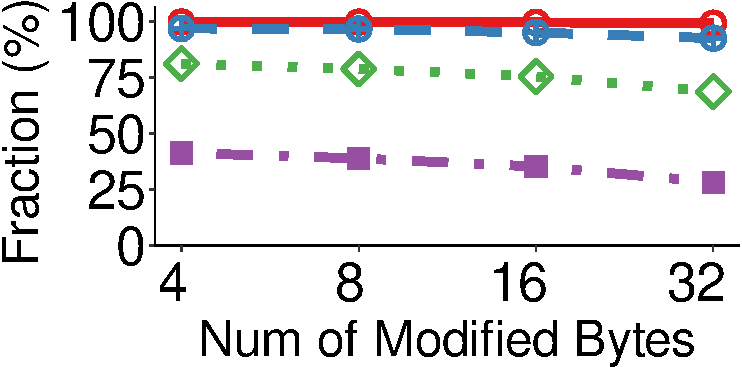
\includegraphics[width=0.45\textwidth]{pic/featurespy/plot/detection/syn/fixed_p_4.pdf} &
        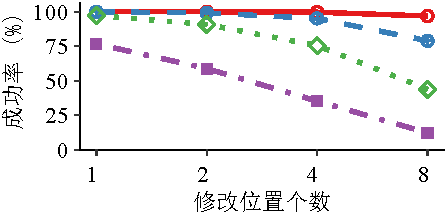
\includegraphics[width=0.45\textwidth]{pic/featurespy/plot/detection/syn/fixed_q_16.pdf}\\
        \mbox{\small (a) Fix $x=4$ and vary $y$}&
        \mbox{\small (b) Fix $y=16$ and vary $x$}\\
    \end{tabular}
    \vspace{-6pt}
    \caption{(Exp\#1) 明文块的相似性检测。 我们评估每个合成数据集 SYNChunk$(x, y)$ 中所有相似块中具有某些相同特征的块的比例。}
    \vspace{-6pt}
    \label{fig:featurespy-expDetectionSynSim}
\end{figure}

图~\ref{fig:featurespy-expDetectionSynSim} 显示了当我们使用具有固定 $x$ = 4 和变化 $y$ 的 SYNChunk$(x, y)$ 时的结果(图~\ref{fig:featurespy-expDetectionSynSim}( a)),以及具有固定的 $y$ = 16 和变化的 $x$(图~\ref{fig:featurespy-expDetectionSynSim}(b))。一般来说,识别出的相似块的比例会随着 $x$ 和 $y$ 而降低,因为重大修改可能会修改块的内容特征。具体来说,该分数受 $x$(比 $y$)的影响更大,因为增加 $x$ 将改变大量滑动窗口(\S\ref{subsec:featurespy-basic})的拉宾指纹。另一方面,我们可以通过检查它们是否共享一个或两个相同的特征来有效地检测大部分(例如,至少 78.9\%)的相似块。



\paragraph*{Exp\#2(密文块的相似性检测)。}
我们扩展 Exp\#1 来研究基于密文块的 \sysnameF 的相似性检测。我们应用我们的设计技术并研究相应操作后相似性保留的有效性。具体来说,我们对每个明文块执行特征密钥生成(通过 \S\ref{subsec:featurespy-spe} 中的建议实例),并评估相似块的比例(在每个合成数据集 SYNChunk$(x, y)$ 中)分配有相同的功能键。然后,我们执行 SPE,并进一步评估可以基于相应(加密)相似性指标识别的相似块的比例。在这里,我们关注三个 SPE 实例 SPE$(1)$、SPE$(2)$ 和 SPE$(4)$,它们划分了第一个、第二个和四个块(分别占用 16、32 和 64 个字节)每个明文块分别作为相似度指标。

\begin{figure*}[t]
    \centering
    
\includegraphics[width=0.4\textwidth]{pic/featurespy/plot/detection/syn/synBarPlotDetect_legend.pdf}\\
    \begin{tabular}{@{}c@{}c@{}c}
        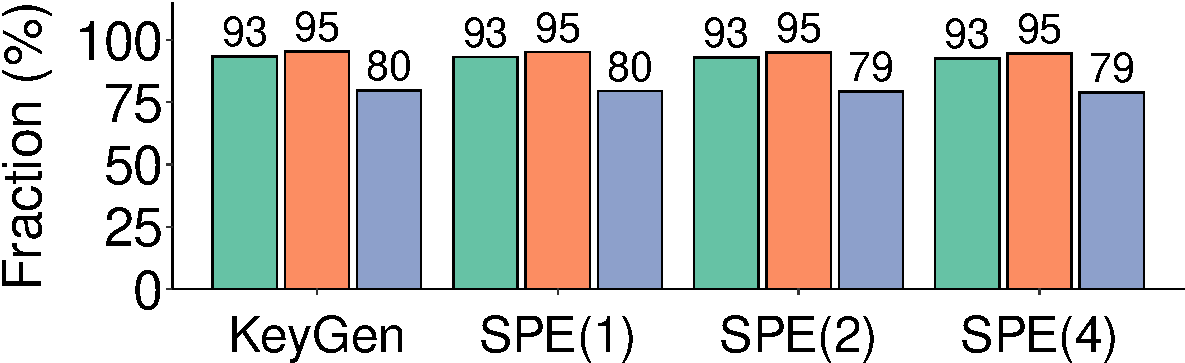
\includegraphics[width=0.32\textwidth]{pic/featurespy/plot/detection/syn/syn-p1-q4-detect.pdf} &
        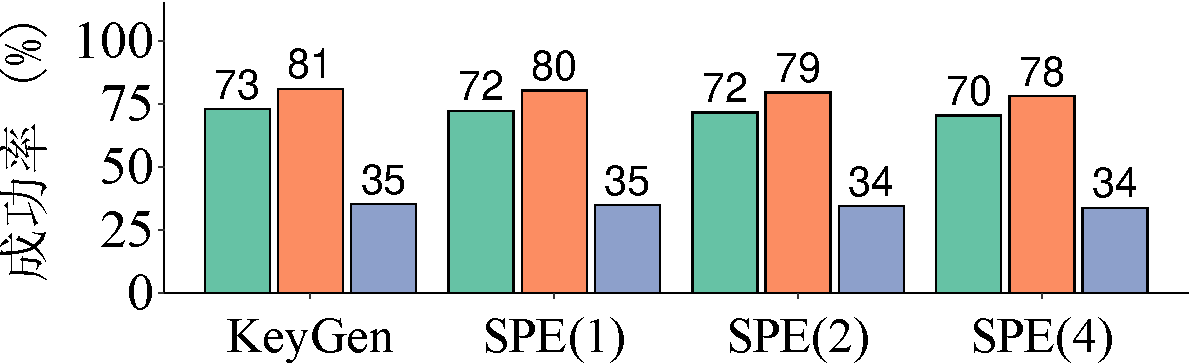
\includegraphics[width=0.32\textwidth]{pic/featurespy/plot/detection/syn/syn-p4-q16-detect.pdf} &
        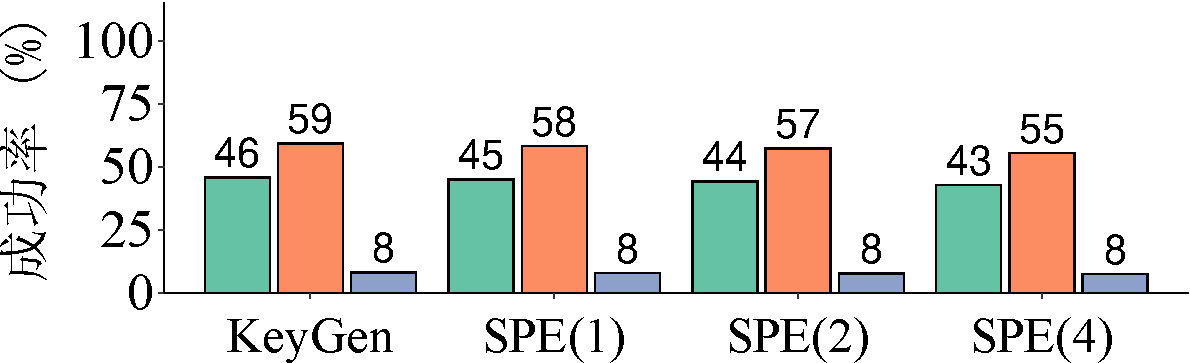
\includegraphics[width=0.32\textwidth]{pic/featurespy/plot/detection/syn/syn-p8-q32-detect.pdf}\\
        \mbox{\small (a) $\textrm{SYNChunk}(1, 4)$}&
        \mbox{\small (b) $\textrm{SYNChunk}(4, 16)$}&
        \mbox{\small (c) $\textrm{SYNChunk}(8, 32)$}\\
    \end{tabular}
    \vspace{-6pt}
    \caption{(Exp\#2) 密文块的相似性检测。 我们评估分配有相同特征键(对于 KeyGen)的相似块的比例,以及可以通过检查相似性指标来检测(对于配置第一个 $i$ 数据块的每个 SPE$(i)$ 每个明文块作为相应的相似性指标)。}
    \vspace{-6pt}
    \label{fig:featurespy-expDetectionSynDetect}
\end{figure*}

图~\ref{fig:featurespy-expDetectionSynDetect} 共同展示了具有小 (SYNChunk$(1, 4)$)、中 (SYNChunk$(4, 16)$) 和大 (SYNChunk$(8, 32)$) 修改相似的块,分别。与 {\tt allFeature} 相比,实例 {\tt firstFeature} 和 {\tt minFeature} 为更相似的块生成相同的特征键,尤其是当修改量很大时(例如,{\tt firstFeature} 和 59.3 的 45.7\% {\tt minFeature} 的 \% 与 {\tt allFeature} 的 8.1\%)。此外,{\tt minFeature} 优于 {\tt firstFeature},这可能是因为最小内容特征对块内容的随机变化更加稳健。此外,我们观察到 SPE 在加密后保留了相似性。具体来说,通过检查密文块中的相似性指标,我们在 SYNChunk$(1, 4)$、SYNChunk$(4, 16)$ 和 SYNChunk$( 8, 32)$,分别。


\paragraph*{Exp\#3(攻击检测案例研究)。}
我们扩展了 \S\ref{subsec:featurespy-attack} 中的案例研究,以研究 \sysnameF 如何检测推断工资和签约奖金的学习内容攻击。我们用一个固定比率阈值 $T$ = 3\% 和一个大小为两个块(或等效 32 字节)的相似性指标配置 \sysnameF。回想一下 \S\ref{subsec:featurespy-attack},对手需要伪造 101 个 $\times$ 31 = 3131 个对抗性提议,其中年薪和签约奖金分别有 101 和 31 个可能值。为了模拟在普通快照中上传对抗提议的对手(否则更容易检测到),我们将所有对抗提议随机插入到每个 Linux/CouchDB 快照中,对 {\em 攻击快照} 的每个单独文件执行分块(即包括对抗性提议)作为现有的基于数据块的重复数据删除方法 \cite{fsl, meyer11},并进一步在块上应用 SPE。我们评估 {\em 检测率},它是 \sysnameF 成功检测到的此类攻击快照的数量与攻击快照总数的比率。此外,我们让 \sysnameF 处理每个原始快照(没有对抗性注入),并评估 {\em false rate},即 \sysnameF 误判的快照数量与原始快照总数的比率。我们展示了 \sysnameF 如何检测学习内容攻击,然后是整体检测结果。 在这里,我们不考虑 FSL 和 MS 进行评估,因为它们没有实际的数据内容。


\begin{figure*}[t]
    \centering
    
\includegraphics[width=0.5\textwidth]{pic/featurespy/plot/detection/overall/prefixDistribution_legend.pdf}\\
    \begin{tabular}{@{\ }c@{\ }c@{\ }c}
        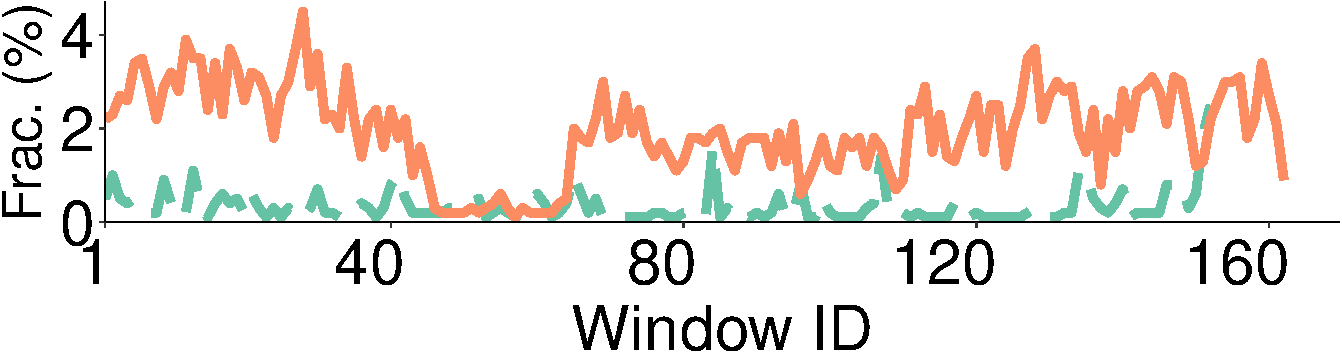
\includegraphics[width=0.32\textwidth]{pic/featurespy/plot/detection/overall/prefixDistribution-1000-Linux-first.pdf} &
        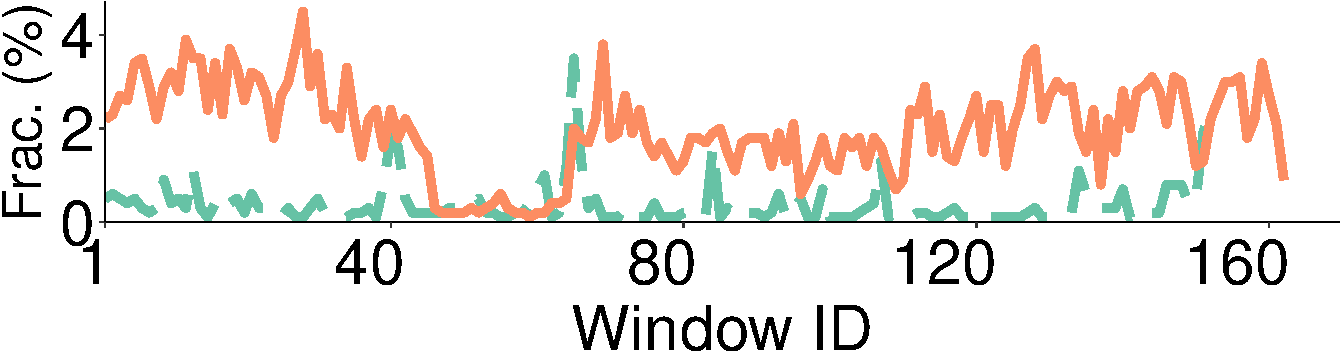
\includegraphics[width=0.32\textwidth]{pic/featurespy/plot/detection/overall/prefixDistribution-1000-Linux-min.pdf} &
        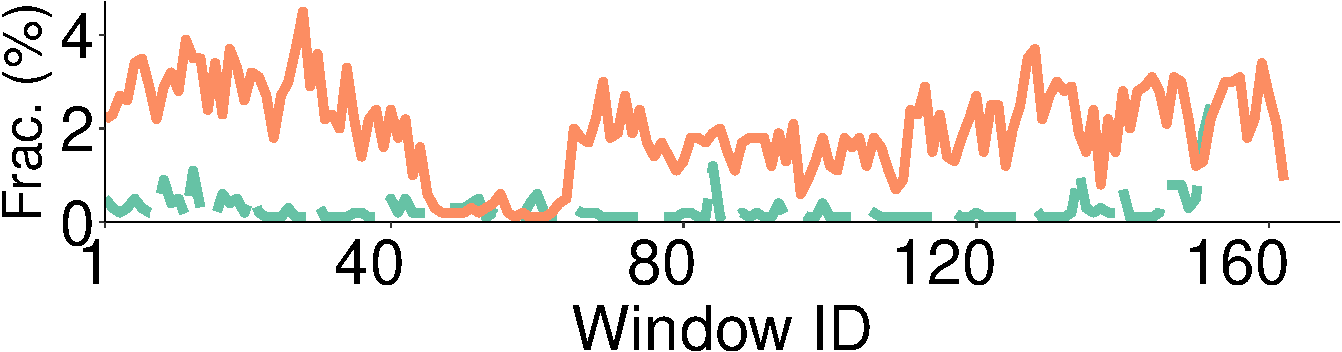
\includegraphics[width=0.32\textwidth]{pic/featurespy/plot/detection/overall/prefixDistribution-1000-Linux-all.pdf} \\
        \mbox{\makecell[c]{\small (a) {\tt firstFeature}}}&
        \mbox{\makecell[c]{\small (b) {\tt minFeature}}}&
        \mbox{\makecell[c]{\small (c) {\tt allFeature}}}\\
    \end{tabular}
    \vspace{-5pt}
    \caption{(Exp\#3) 一个攻击检测示例,显示 {\tt firstFeature}、{\tt minFeature} 和 {\tt allFeature} 处理具有(即攻击)和不具有(即原始)的相同 Linux 快照 对抗性注射。 我们展示了在每个窗口中具有相同相似性指标的最多块数占块总数(固定为 $W$ = 1\,K)的比例。}
    \label{fig:featurespy-expDetectionOverall}
  \end{figure*}

  图~\ref{fig:featurespy-expDetectionOverall} 比较 \sysnameF 实例在检测相同 Linux 快照(即 v5.13)中注入(即攻击)或没有(即原始)对抗性提议的学习内容攻击.具体来说,x 轴索引处理窗口(其大小在此处固定为 1\,K),而 y 轴显示 {\em most} 数量的密文块中具有相同相似性指示符的部分相应窗口中所有块的总数(即 1\,K)。我们观察到所有三个实例都可以有效地检测到学习内容攻击,因为它们在攻击快照中至少有一个窗口,因此具有相同相似性指标的密文块的比例大于 $T $(即 3\%)。另一方面,{\tt minFeature} 遭受 {\em false positive},因为它甚至有一个正常的窗口(例如,原始的第 65 个窗口),其中分数(例如,3.5\%)检测到相似的块中大于$T$。


\begin{figure}[t]
    \centering
    
\includegraphics[width=0.5\textwidth]{pic/featurespy/plot/detection/overall/effectiveness-falsePositive_legend.pdf}
    \vspace{5pt}\\
    \begin{tabular}{@{\ }c@{\ }c}
        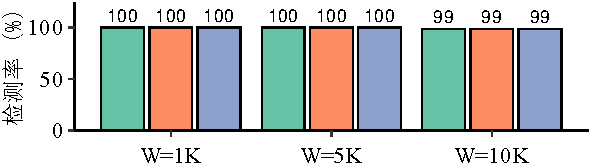
\includegraphics[width=0.6\textwidth]{pic/featurespy/plot/detection/overall/effectivenessLinux.pdf} &
        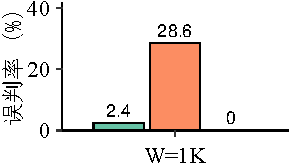
\includegraphics[width=0.3\textwidth]{pic/featurespy/plot/detection/overall/falsePositiveLinux.pdf}\\
        \mbox{\small (a) Detection rate} &
        \mbox{\small (b) False rate}\\
    \end{tabular}
    \vspace{-6pt}
    \caption{(Exp\#3) 每个 Linux 快照中的总体检测率和错误率。 请注意,{\tt allFeature} 没有任何误报。}
    \vspace{-6pt}
    \label{fig:featurespy-expDetectionOverallFalsePositive}
\end{figure}

图~\ref{fig:featurespy-expDetectionOverallFalsePositive} 展示了我们将窗口大小分别配置为 1\,K, 5\,K 和 10\,K 时 Linux 中的总体检测率和误报率。通常,\sysnameF 在 Linux 快照中实现了很高的检测率(例如,至少 98.6\%)。然而,较大的窗口会略微降低检测率,因为相对较小部分的密文块具有相同的相似性指标。
此外,\sysnameF 仅在窗口大小为 1\,K 时才会产生误报(图~\ref{fig:featurespy-featureDistribution}(b)),因为原始快照最初具有相当大的部分相似块。即使在这种情况下,{\tt allFeature} 也没有任何误报,因为它只检测到少量相似的块。另一方面,检测到更多相似块 (Exp\#2) 的 {\tt minFeature} 会产生 28.6\% 的误报。


除了 Linux,我们在 CouchDB 中评估 \sysnameF 并发现所有 \sysnameF 实例成功检测到所有 CouchDB 快照中的学习内容攻击(即 100\% 的检测率),而没有引入任何误报。可能的原因是每个 CouchDB 快照都有许多不相似的块,当注入许多对抗性的相似块时,\sysnameF 可以立即检测到(相似块的)分布变化。


\paragraph*{Exp\#4(不同目标文件的影响)。}
我们现在研究 \sysnameF 在用于检测针对每个合成文件 SYNFile$(x, y)$ 的学习内容攻击时的有效性(回想一下,$x$ 是文件中未知变量的数量,$y $ 是每个变量的可能值的数量)。为了攻击 SYNFile$(x, y)$,我们枚举了 $x\times y$ 对抗文件,将它们随机插入到最后一个 Linux 快照(最大大小为 985.9\,MiB 以及其他快照)中,并评估检测运行 100 次后 \sysnameF 的速率(配置为固定的 $T$ = 3\%)。


\begin{figure}[t]
    \centering
    
\includegraphics[width=0.5\textwidth]{pic/featurespy/plot/detection/trade-off/trade_off_legend.pdf}
    \vspace{5pt}\\
    \begin{tabular}{@{\ }c@{\ }c@{\ }c}
        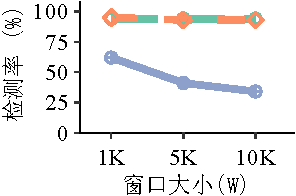
\includegraphics[width=0.32\textwidth]{pic/featurespy/plot/detection/trade-off/varyWindow_linux.pdf} &
        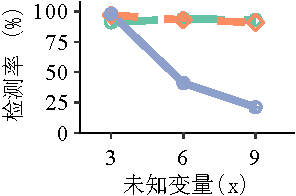
\includegraphics[width=0.32\textwidth]{pic/featurespy/plot/detection/trade-off/varyModifyPos_linux.pdf}&
        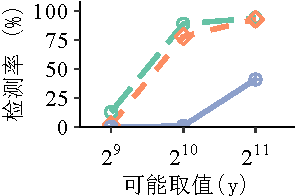
\includegraphics[width=0.32\textwidth]{pic/featurespy/plot/detection/trade-off/varyFileNumber_linux.pdf} \\
        \makecell[c]{\small (a) Vary $W$ \\ \small against SYNFile$(6, 2048)$} &
        \makecell[c]{\small (b) Fix W = 5\,K \\ \small against SYNFile$(\cdot, 2048)$} &
        \makecell[c]{\small (c) Fix W = 5\,K \\ \small against SYNFile$(6, \cdot)$} \\
    \end{tabular}
    \vspace{-6pt}
    \caption{(Exp\#4) Impact of different target files.}
    \vspace{-6pt}
    \label{fig:featurespy-expDetectionTradeOff}
\end{figure}

图~\ref{fig:featurespy-expDetectionTradeOff}(a) 展示了当我们改变窗口大小 $W$ 来攻击 SYNFile$(6, 2048)$ 时的结果。 {\tt firstFeature} 和 {\tt minFeature} 的检测率对 $W$ 的增加是稳健的(例如,始终保持在 93\% 以上),但 {\tt allFeature} 的检测率下降到 34\%。原因是 {\tt allFeature} 只能检测到少量相似的块(Exp\#2),当 $W$ 很大时,这些块的比例很低。图~\ref{fig:featurespy-expDetectionTradeOff}(b) 展示了我们改变目标文件中未知变量 $x$ 的数量时的结果。我们观察到,当 $x$ = 9 时,{\tt allFeature} 的检测率再次急剧下降到 21\%,因为它无法检测到具有更多不同区域的相似块。


图~\ref{fig:featurespy-expDetectionTradeOff}(c) 展示了当我们改变目标文件中每个变量的可能值的数量 $y$ 时的结果。当 $y$ 为 512 时,所有三个实例的检测率都较低(例如,高达 13\%)。原因是目标文件的熵较低,攻击者只需要构建少量相似的内容。 \sysnameF 在这种情况下检测学习内容攻击是无效的。 一种可能的解决方案是配置一个小的 $T$ 或 $W$ 以在检测到几个类似的块时报告攻击案例,但这会增加在不同工作负载中误判的可能性。 我们提出了一项未来的工作,即如何自动平衡检测对低熵文件的攻击和在处理不同工作负载时最大限度地减少误判之间的权衡。